\documentclass{beamer}
\useoutertheme[right]{sidebar}
\setbeamertemplate{items}[square]
\setbeamertemplate{navigation symbols}{}

%\setbeamertemplate{footline}[frame number]

\setbeamercolor{frametitle}{fg=white,bg=red!50!black}
\setbeamercolor{sidebar}{bg=black!20}
\setbeamercolor{logo}{bg=red!30!black}
\setbeamercolor{section in sidebar}{fg=white}            %color of the active section
\setbeamercolor{section in sidebar shaded}{fg=black!50}     %color of the inactive section
\setbeamercolor{subsection in sidebar}{fg=white}         %color of the active subsection
\setbeamercolor{subsection in sidebar shaded}{fg=black!40}  %color of the inactive subsection
\setbeamercolor{title}{fg=white,bg=red!50!black}
\setbeamercolor{itemize item}{fg=red!50!black}
\setbeamercolor{itemize subitem}{fg=red!50!black}
\setbeamercolor{itemize subsubitem}{fg=red!50!black}
%\setbeamercolor{author}{fg=white}
%\setbeamercolor{institute}{fg=white}
%\setbeamercolor{date}{fg=white}

\setbeamertemplate{sidebar right}
{
  \insertverticalnavigation{\swidth}
  \vfill
  \hbox to2cm{\hskip0.6cm\usebeamerfont{subsection in sidebar shaded}
   \strut\usebeamercolor[fg]{subsection in
      sidebar shaded}\insertframenumber / \inserttotalframenumber\hfill}
  \vskip3pt
}

\usepackage{multicol}
\newcommand{\pd}[2]{\frac{\partial #1}{\partial #2}}
\newcommand{\x}{\mathbf{x}}
\newcommand{\xt}{(\x,t)}
\renewcommand{\ij}{_{i,j}}
\newcommand{\U}{\mathbf{U}}
\newcommand{\M}{\mathbf{M}}
\newcommand{\A}{\mathbf{A}}
\newcommand{\D}{\mathbf{D}}
\newcommand{\F}{\mathbf{F}}
\renewcommand{\L}{\mathcal{L}}
\newcommand{\f}{\mathbf{f}}
\renewcommand{\b}{\mathbf{b}}
\newcommand{\dt}{\Delta t}

\title[]{A Positivity-Preserving Flux-Corrected Transport Scheme
Using Continuous Finite Elements} 
\author[]{Joshua E. Hansel\inst{1} \and Jean C. Ragusa\inst{1}
   \and Jean-Luc Guermond\inst{2}}
\institute{
  \inst{1}Department of Nuclear Engineering\\
   Texas A\&M University
   \and
   \inst{2}Department of Mathematics\\
   Texas A\&M University}
\date[Summer 2015]{Idaho National Laboratory, Summer 2015}
\logo{
\includegraphics[height=0.1\textwidth]{./figures/TAMU-Logo-white.png}}

\begin{document}
%%%%%%%%%%%%%%%%%%%%%%%%%%%%%%%%%%%%%%%%%%%%%%%%%%%%%%%%%%%%%%%%%%%%%%%%%%%%%%%%%%%%%%%%%%%%%
{
\setbeamercolor{background canvas}{bg=black!10}
\begin{frame}[plain]
   % remove space reserved for sidebar
   \advance\textwidth1.5cm
   \hsize\textwidth
   \columnwidth\textwidth
	
   \titlepage
\end{frame}
}
%%%%%%%%%%%%%%%%%%%%%%%%%%%%%%%%%%%%%%%%%%%%%%%%%%%%%%%%%%%%%%%%%%%%%%%%%%%%%%%%%%%%%%%%%%%%%
\section{Introduction}
\subsection{Motivation}
\begin{frame}
\frametitle{Motivation}

\begin{itemize}
   \item Numerical solution of transport equation prone to spurious oscillations
   and negativities in regions of discontinuities and sharp gradients:
   \begin{center}
      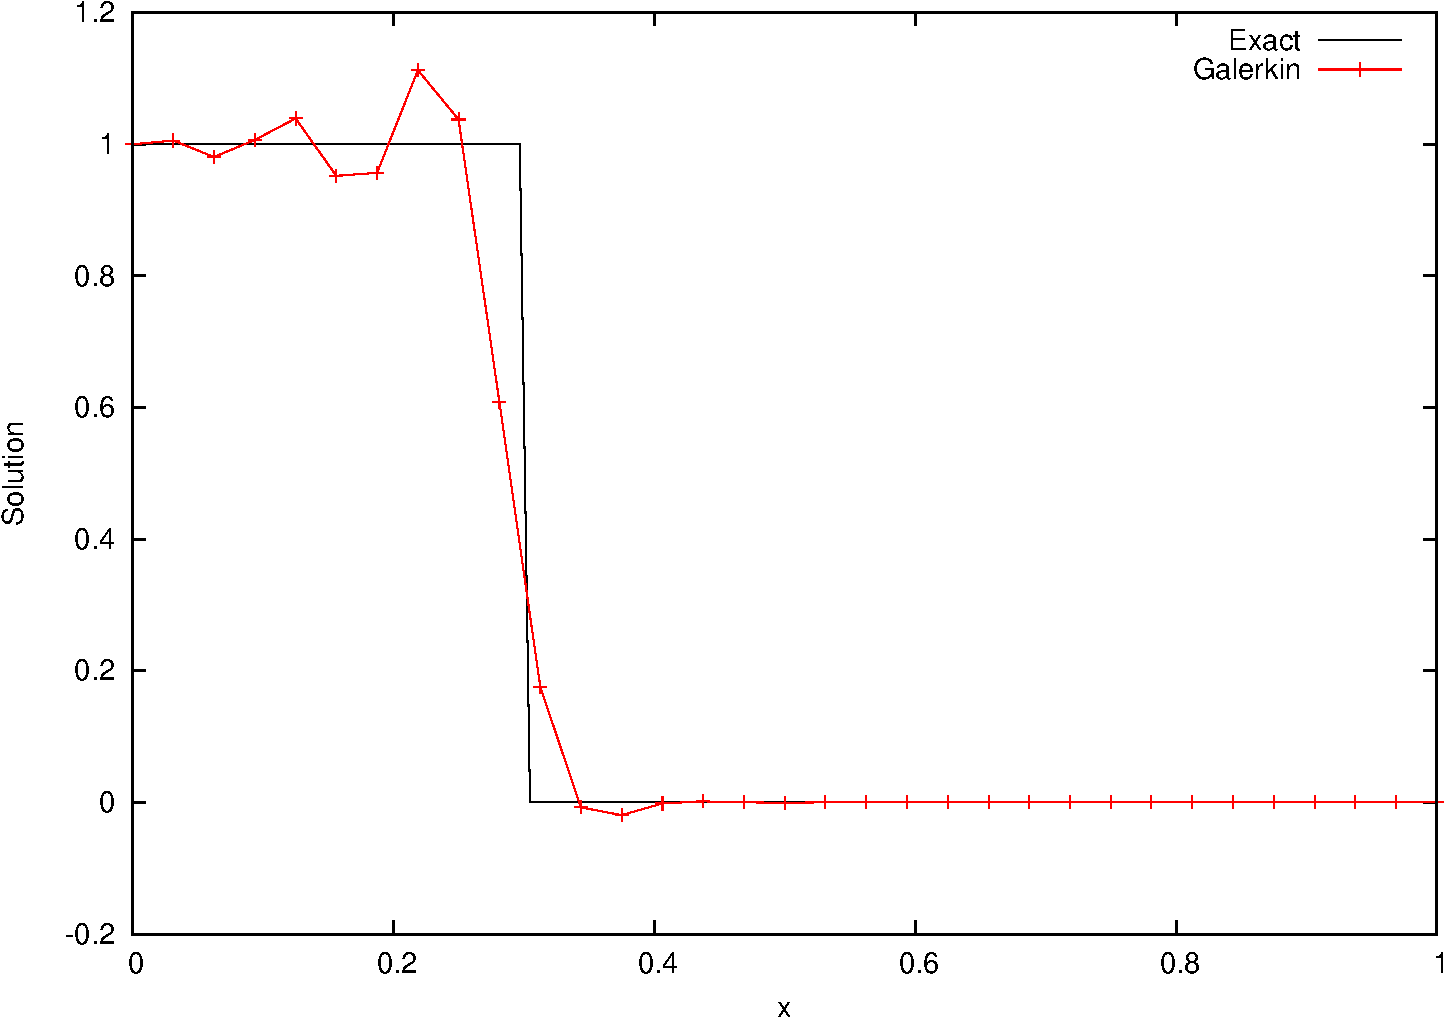
\includegraphics[width=0.7\textwidth]{./figures/advection_Galerkin.pdf}
   \end{center}
\end{itemize}

\end{frame}
%%%%%%%%%%%%%%%%%%%%%%%%%%%%%%%%%%%%%%%%%%%%%%%%%%%%%%%%%%%%%%%%%%%%%%%%%%%%%%%%%%%%%%%%%%%%%
\subsection{Objective and Plan}
\begin{frame}
\frametitle{Objective and Plan}

\begin{itemize}
   \item The \textbf{Objective} is to obtain a solution to the transport equation that
      \begin{itemize}
         \item uses CFEM - not a traditional discretization for transport,
            but recent efforts have used CFEM for shock hydrodynamics
         \item is non-negative
         \item is free of spurious oscillations
         \item has high-order accuracy (2nd order)
      \end{itemize}
   \item The \textbf{Plan} is the following:
   \begin{itemize}
      \item Use a low-order, monotone, non-negative scheme in conjunction with
      a high-order scheme via the flux-corrected transport (FCT) algorithm
      to produce a high-order, non-negative scheme
      \begin{itemize}
         \item monotonicity not guaranteed but demonstrated for most cases
      \end{itemize}
   \end{itemize}
\end{itemize}

\end{frame}
%%%%%%%%%%%%%%%%%%%%%%%%%%%%%%%%%%%%%%%%%%%%%%%%%%%%%%%%%%%%%%%%%%%%%%%%%%%%%%%%%%%%%%%%%%%%%
\section{Methodology}
\subsection{Problem Formulation}
\begin{frame}
\frametitle{Problem Formulation}

\begin{itemize}
   \item Model transport equation:
   \begin{align}\label{eq:tr}
      &\frac{1}{v}\pd{\psi}{t} + \mathbf{\Omega}\cdot\nabla \psi\xt
      + \Sigma(\x)\psi\xt = q\xt\\
      &\Sigma(\x)\ge 0,\qquad q\xt\ge 0\nonumber
   \end{align}
   \item Define problem:
   \begin{equation}
      \psi(\x,0) = \psi^0(\x) \quad \forall \x\in \mathcal{D}
   \end{equation}
   \begin{equation}
      \psi\xt = \psi^{inc}(\x) \quad \forall \x\in \partial \mathcal{D}^{inc}
   \end{equation}
   \item CFEM solution:
   \begin{equation}
      \psi_h\xt = \sum\limits_{j=1}^N U_j(t) \varphi_j(\x),
      \quad \varphi_j(\x)\in P^1_h
   \end{equation}
\end{itemize}

\end{frame}
%%%%%%%%%%%%%%%%%%%%%%%%%%%%%%%%%%%%%%%%%%%%%%%%%%%%%%%%%%%%%%%%%%%%%%%%%%%%%%%%%%%%%%%%%%%%%
\subsection{Temporal Discretization}
\begin{frame}
\frametitle{Temporal Discretization}

\begin{itemize}
   \item Fully explicit temporal schemes used here:
   \begin{itemize}
      \item Forward Euler (FE)
      \item Explicit Strong Stability Preserving Runge-Kutta methods,
         which can be expressed as a number of FE steps
   \end{itemize}
   \item Forward Euler scheme:
   \begin{equation}\label{eq:exgalerkin}
      \M^C\frac{\U^{n+1}-\U^n}{\dt} + \A\U^n = \b^n
   \end{equation}
   \begin{equation}
      M\ij^C \equiv \int\limits_{S\ij}\varphi_i(\x) \varphi_j(\x) d\x
   \end{equation}
   \begin{equation}
      A\ij \equiv v\int\limits_{S\ij}\left(
      \mathbf{\Omega}\cdot\nabla\varphi_j(\x) +
		\Sigma(\x)\varphi_j(\x)\right)\varphi_i(\x) d\x
   \end{equation}
   \begin{equation}
      b_i^n \equiv v\int\limits_{S_i} q(\x,t^n)\varphi_i(\x) d\x
   \end{equation}
\end{itemize}

\end{frame}
%%%%%%%%%%%%%%%%%%%%%%%%%%%%%%%%%%%%%%%%%%%%%%%%%%%%%%%%%%%%%%%%%%%%%%%%%%%%%%%%%%%%%%%%%%%%%
\subsection{Low-Order Scheme}
\begin{frame}
\frametitle{Low-Order Scheme}
\framesubtitle{Definition}

\begin{itemize}
   \item Lump mass matrix and add artificial viscosity:
   \begin{equation}\label{eq:loworderscheme}
      \M^L\frac{\U^{L,n+1}-\U^n}{\dt} + (\A + \D^L)\U^n = \b^n
   \end{equation}
   \begin{equation}\label{eq:loworderD}
      D\ij^L = \sum\limits_{K\subset S\ij}\nu_K^L b_K(\varphi_j,\varphi_i)
   \end{equation}
   \begin{equation}\label{eq:bilinearform}
      b_K(\varphi_j, \varphi_i) \equiv \left\{\begin{array}{l l}
         -\frac{1}{n_K - 1}|K| & i\ne j, \quad i,j\in \mathcal{I}(K)\\
         |K|                   & i = j,  \quad i,j\in \mathcal{I}(K)\\
         0                     & i\notin\mathcal{I}(K)\,|\, j\notin\mathcal{I}(K)
      \end{array}\right.
   \end{equation}
   \begin{equation}
      \nu_K^L \equiv \max\limits_{i\ne j\in \mathcal{I}(K)}\frac{\max(0,A\ij)}
      {-\sum\limits_{T\subset S\ij} b_T(\varphi_j, \varphi_i)}
   \end{equation}
\end{itemize}

\end{frame}
%%%%%%%%%%%%%%%%%%%%%%%%%%%%%%%%%%%%%%%%%%%%%%%%%%%%%%%%%%%%%%%%%%%%%%%%%%%%%%%%%%%%%%%%%%%%%
\begin{frame}
\frametitle{Low-Order Scheme}
\framesubtitle{Properties}

\begin{itemize}
   \item These definitions make $(\A + \D^L)$ an M-matrix, which has
      the following desirable consequences for the low-order solution $\U^{L,n+1}$:
   \begin{itemize}
      \item monotonicity
      \item non-negativity
      \item satisfaction of a discrete maximum principle (DMP):
      \begin{equation}\label{eq:dmp}
         W_i^-(\U^n)\leq
         U_i^{L,n+1}\leq
         W_i^+(\U^n)\qquad\forall i
      \end{equation}
      \begin{equation}
         W_i^\pm(\U^n) \equiv U_{\substack{\max\\\min},i}^n\left(1-\frac{\dt}{m_i}
         \sum\limits_j A\ij^L\right)
         + \frac{\Delta t}{m_i}b_i^n
      \end{equation}
   \end{itemize}
   \item Undesirable consequence: first-order accuracy
\end{itemize}

\end{frame}
%%%%%%%%%%%%%%%%%%%%%%%%%%%%%%%%%%%%%%%%%%%%%%%%%%%%%%%%%%%%%%%%%%%%%%%%%%%%%%%%%%%%%%%%%%%%%
\begin{frame}
\frametitle{Low-Order Scheme}
\framesubtitle{Results Example}

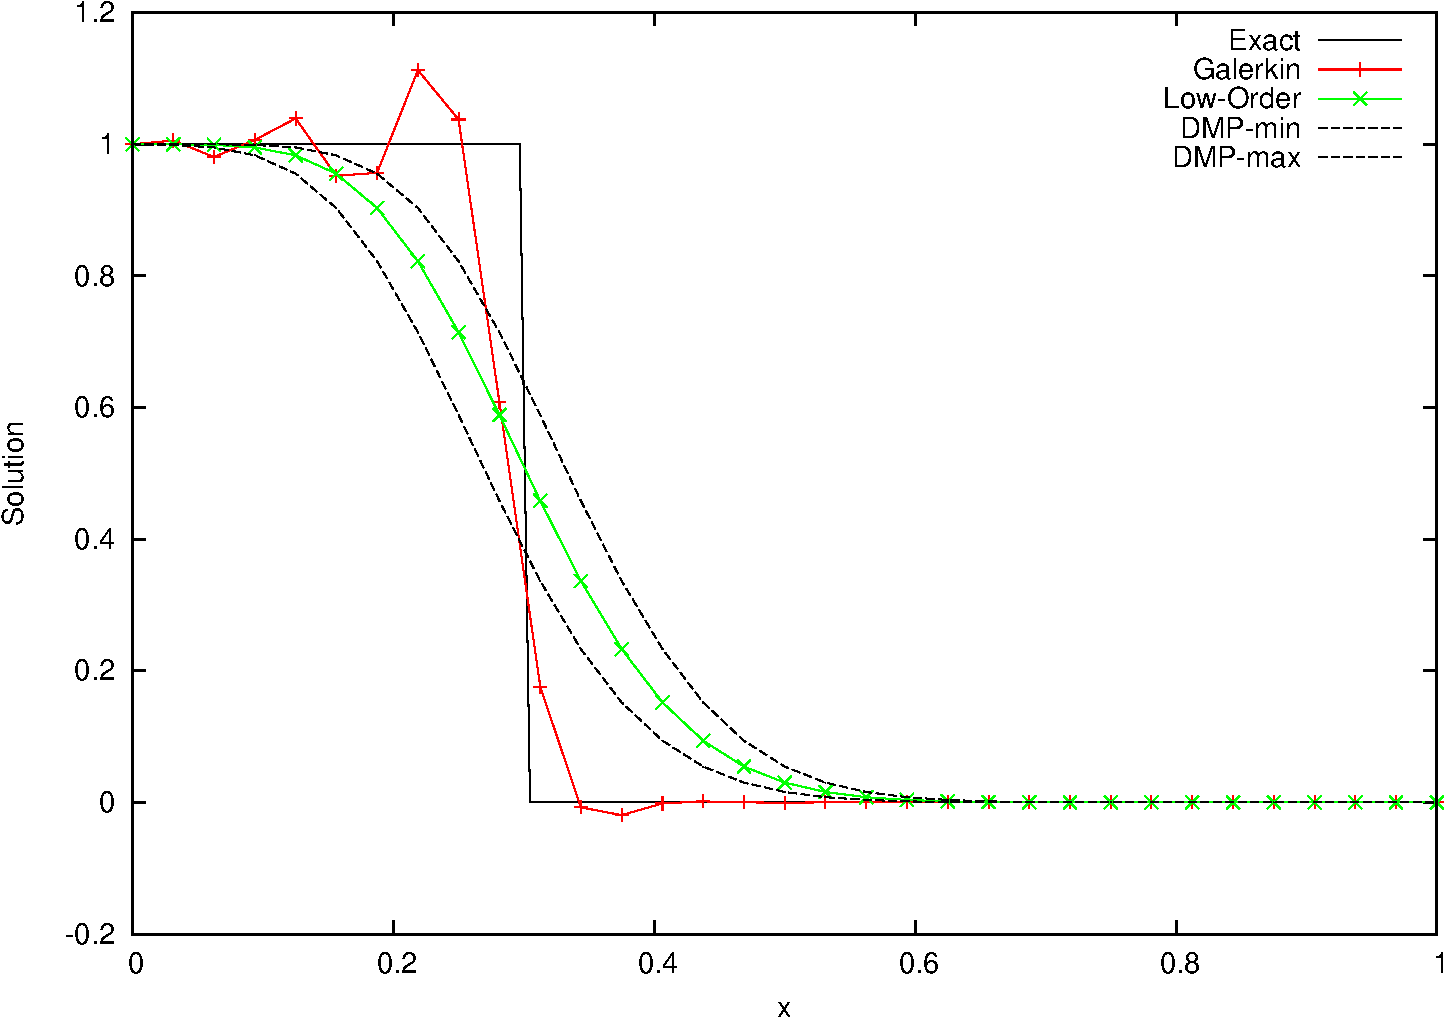
\includegraphics[width=\textwidth]{./figures/advection_low_order.pdf}

\end{frame}
%%%%%%%%%%%%%%%%%%%%%%%%%%%%%%%%%%%%%%%%%%%%%%%%%%%%%%%%%%%%%%%%%%%%%%%%%%%%%%%%%%%%%%%%%%%%%
\subsection{High-Order Scheme}
\begin{frame}
\frametitle{High-Order Scheme}
\framesubtitle{Definition}

\begin{itemize}
   \item Add high-order artificial viscosity:
   \begin{equation}
      \M^C\frac{\U^{H,n+1}-\U^n}{\dt} + (\A + \D^{H,n})\U^n = \b^n
   \end{equation}
   \begin{equation}
      D\ij^{H,n} = \sum\limits_{K\subset S\ij}\nu_K^{H,n} b_K(\varphi_j,\varphi_i)
   \end{equation}
   \begin{equation}
      \nu^{H,n}_K = \min(\nu^{L}_K,\nu^{E,n}_K)
   \end{equation}
   \item The entropy-based artificial viscosity $\nu^{E,n}_K$ is
   proportional to local ``entropy'' production.
\end{itemize}

\end{frame}
%%%%%%%%%%%%%%%%%%%%%%%%%%%%%%%%%%%%%%%%%%%%%%%%%%%%%%%%%%%%%%%%%%%%%%%%%%%%%%%%%%%%%%%%%%%%%
\begin{frame}
\frametitle{High-Order Scheme}
\framesubtitle{Entropy Viscosity Definition}

\begin{itemize}
   \item One chooses a convex entropy function $E(\psi)$ such
   as $E(\psi)=\frac{1}{2}\psi^2$ and manipulates the
   transport equation to get an entropy residual:
   \begin{equation}
      R_K(\psi) = \left\|\pd{E}{t}
      + \frac{dE}{d\psi}\left(\mathbf{\Omega}\cdot\nabla \psi
      + \sigma \psi
      - q \right)\right\|_{L^\infty(K)}
   \end{equation}
   \item Entropy-based artificial viscosity is proportional to an entropy
   residual $R_K^n(\psi_h)$:
   \begin{equation}
      \nu^{E,n}_K = \frac{c_E R_K^n(\psi_h)
      + c_J\max\limits_{F\in\partial K}J_F(\psi_h^n)}
      {\|E(\psi_h^n)-\bar{E}(\psi_h^n)\|_{L^\infty(\mathcal{D})}}
   \end{equation}
\end{itemize}
   
\end{frame}
%%%%%%%%%%%%%%%%%%%%%%%%%%%%%%%%%%%%%%%%%%%%%%%%%%%%%%%%%%%%%%%%%%%%%%%%%%%%%%%%%%%%%%%%%%%%%
\begin{frame}
\frametitle{High-Order Scheme}
\framesubtitle{Results Example}

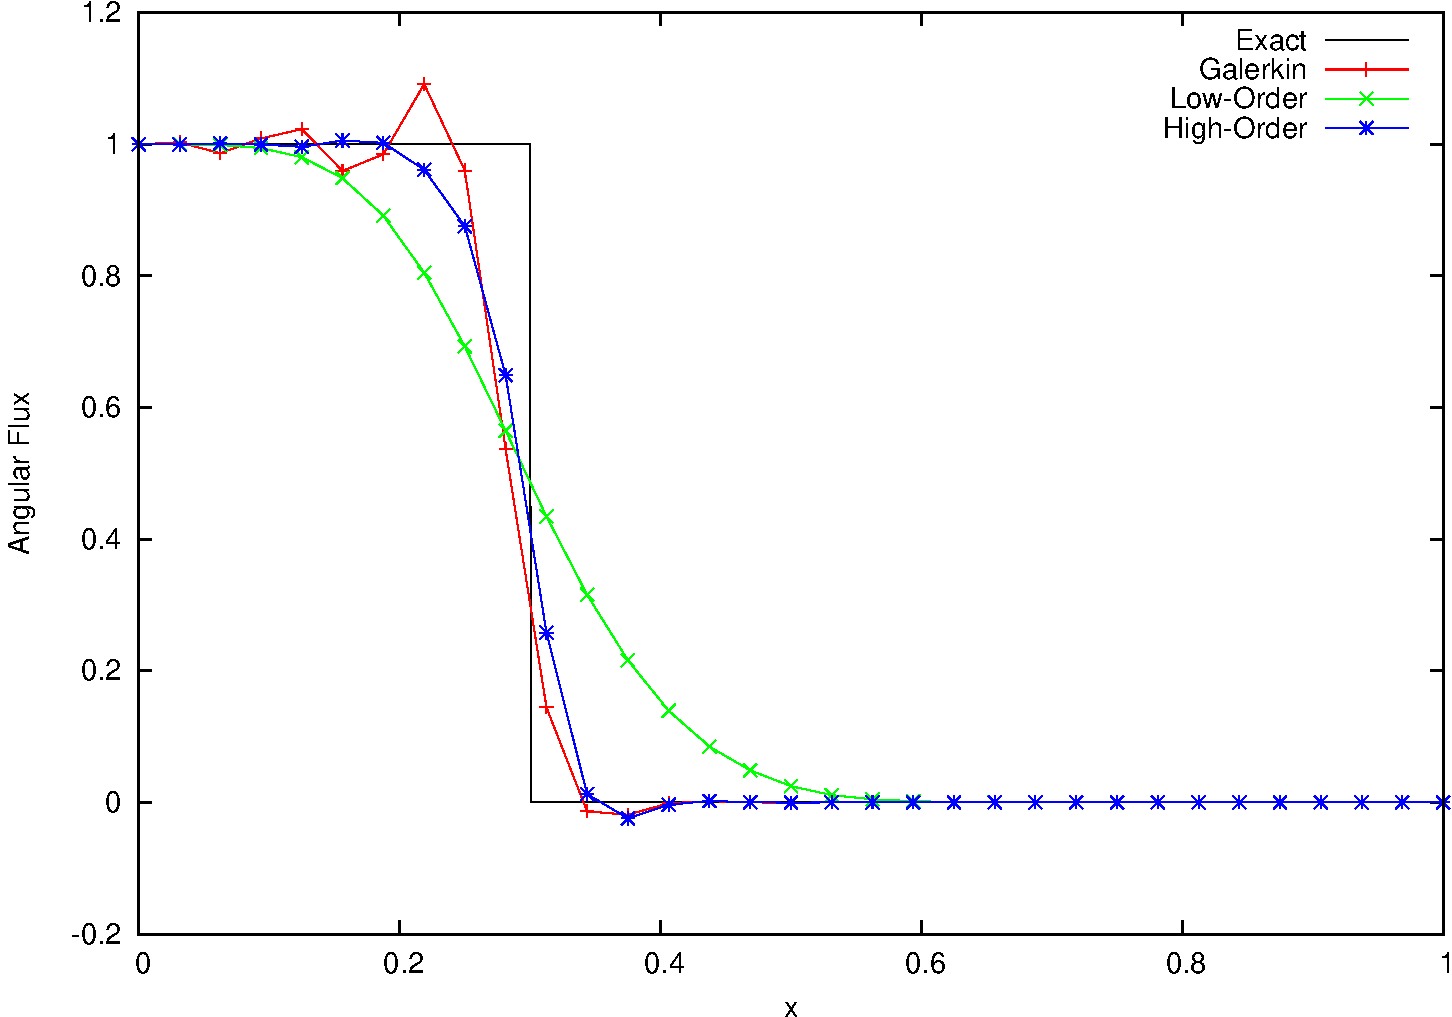
\includegraphics[width=\textwidth]{./figures/advection_high_order.pdf}

\end{frame}
%%%%%%%%%%%%%%%%%%%%%%%%%%%%%%%%%%%%%%%%%%%%%%%%%%%%%%%%%%%%%%%%%%%%%%%%%%%%%%%%%%%%%%%%%%%%%
\subsection{FCT Scheme}
\begin{frame}
\frametitle{Flux Corrected Transport (FCT) Scheme}
\framesubtitle{Introduction}

\begin{itemize}
   \item Initially developed in 1973 for finite difference discretizations of
      transport/conservation law problems and recently applied to finite element method
   \item Works by adding conservative fluxes to satisfy physical bounds on the solution
   \item Employs low-order scheme and high-order scheme
   \item Defines a \emph{correction}, or \emph{antidiffusion}, flux, which
      when added to the low-order scheme, produces the high-order scheme
   \item Limits this correction flux to enforce the physical bounds imposed
\end{itemize}

\end{frame}
%%%%%%%%%%%%%%%%%%%%%%%%%%%%%%%%%%%%%%%%%%%%%%%%%%%%%%%%%%%%%%%%%%%%%%%%%%%%%%%%%%%%%%%%%%%%%
\begin{frame}
\frametitle{Flux Corrected Transport (FCT) Scheme}
\framesubtitle{Correction Flux Definition}

\begin{itemize}
   \item Define a correction flux $\f$:
   \begin{align*}
      \f\,\mbox{Def.:}\quad   & \M^L\frac{\U^{H,n+1}-\U^n}{\dt}+(\A+\D^L)\U^n = \b^n + \f^n\\
      \mbox{Low-order:}\quad  & \M^L\frac{\U^{L,n+1}-\U^n}{\dt}+(\A + \D^L)\U^n = \b^n\\
      \mbox{High-order:}\quad & \M^C\frac{\U^{H,n+1}-\U^n}{\dt}+(\A + \D^{H,n})\U^n = \b^n
   \end{align*}
   \item Thus $\f$ is
   \begin{equation}
      \f^n \equiv -(\M^C-\M^L)\frac{\U^{H,n+1}-\U^n}{\dt} +(\D^L-\D^{H,n})\U^n
   \end{equation}
\end{itemize}

\end{frame}
%%%%%%%%%%%%%%%%%%%%%%%%%%%%%%%%%%%%%%%%%%%%%%%%%%%%%%%%%%%%%%%%%%%%%%%%%%%%%%%%%%%%%%%%%%%%%
\begin{frame}
\frametitle{Flux Corrected Transport (FCT) Scheme}
\framesubtitle{FCT Overview}

\begin{itemize}
   \item Decompose $\f$ into internodal fluxes $F\ij$: $f_i = \sum\limits_j F\ij$:
   \begin{multline}
      F\ij = -M\ij^C\left(\frac{dU_j}{dt}^{H,n+1} - \frac{dU_i}{dt}^{H,n+1}\right)\\
      + (D\ij^L-D\ij^H)(U^n_j - U^n_i)
   \end{multline}
   \item The FCT scheme limits these fluxes with a limiter $\L$:
   \begin{equation}
      \M^L\frac{\U^{n+1}-\U^n}{\dt} + \A^L\U^n = \b + \L[\F]
   \end{equation}
   \item The limiter $\L$ enforces the discrete maximum principle:
   \begin{equation}\label{eq:dmp}
         W_i^-(\U^n)\leq
         U_i^{n+1}\leq
         W_i^+(\U^n)\qquad\forall i
   \end{equation}
\end{itemize}

\end{frame}
%%%%%%%%%%%%%%%%%%%%%%%%%%%%%%%%%%%%%%%%%%%%%%%%%%%%%%%%%%%%%%%%%%%%%%%%%%%%%%%%%%%%%%%%%%%%%
\begin{frame}
\frametitle{Flux Corrected Transport (FCT) Scheme}
\framesubtitle{Limiting Coefficient Definition}

\begin{itemize}
   \item Each correction flux $F\ij$ has an associated limiting
   coefficient $\L\ij$: $\L[\F]_i = \sum\limits_j \L\ij F\ij$:
\begin{equation}\label{eq:P_defs}
   P_i^+ \equiv \sum\limits_j\max(0,F_{i,j}) \qquad
   P_i^- \equiv \sum\limits_j\min(0,F_{i,j})
\end{equation}
\begin{equation}\label{eq:Q_defs}
      Q_i^\pm \equiv m_i\frac{W_i^\pm-U_i^n}{\Delta t}
      + \sum\limits_j A_{i,j}^L U_j^n - b_i
\end{equation}
\begin{equation}\label{eq:R_defs}
   R_i^\pm \equiv\left\{
      \begin{array}{l l}
         1                                          & P_i^\pm = 0\\
         \min\left(1,\frac{Q_i^\pm}{P_i^\pm}\right) & P_i^\pm \ne 0
      \end{array}
      \right.
\end{equation}
\begin{equation}
   \L\ij \equiv\left\{
      \begin{array}{l l}
         \min(R_i^+,R_j^-) & F_{i,j} \geq 0\\
         \min(R_i^-,R_j^+) & F_{i,j} < 0
      \end{array}
      \right.
\end{equation}
\end{itemize}

\end{frame}
%%%%%%%%%%%%%%%%%%%%%%%%%%%%%%%%%%%%%%%%%%%%%%%%%%%%%%%%%%%%%%%%%%%%%%%%%%%%%%%%%%%%%%%%%%%%%
\begin{frame}
\frametitle{Flux Corrected Transport (FCT) Scheme}
\framesubtitle{Results Example}

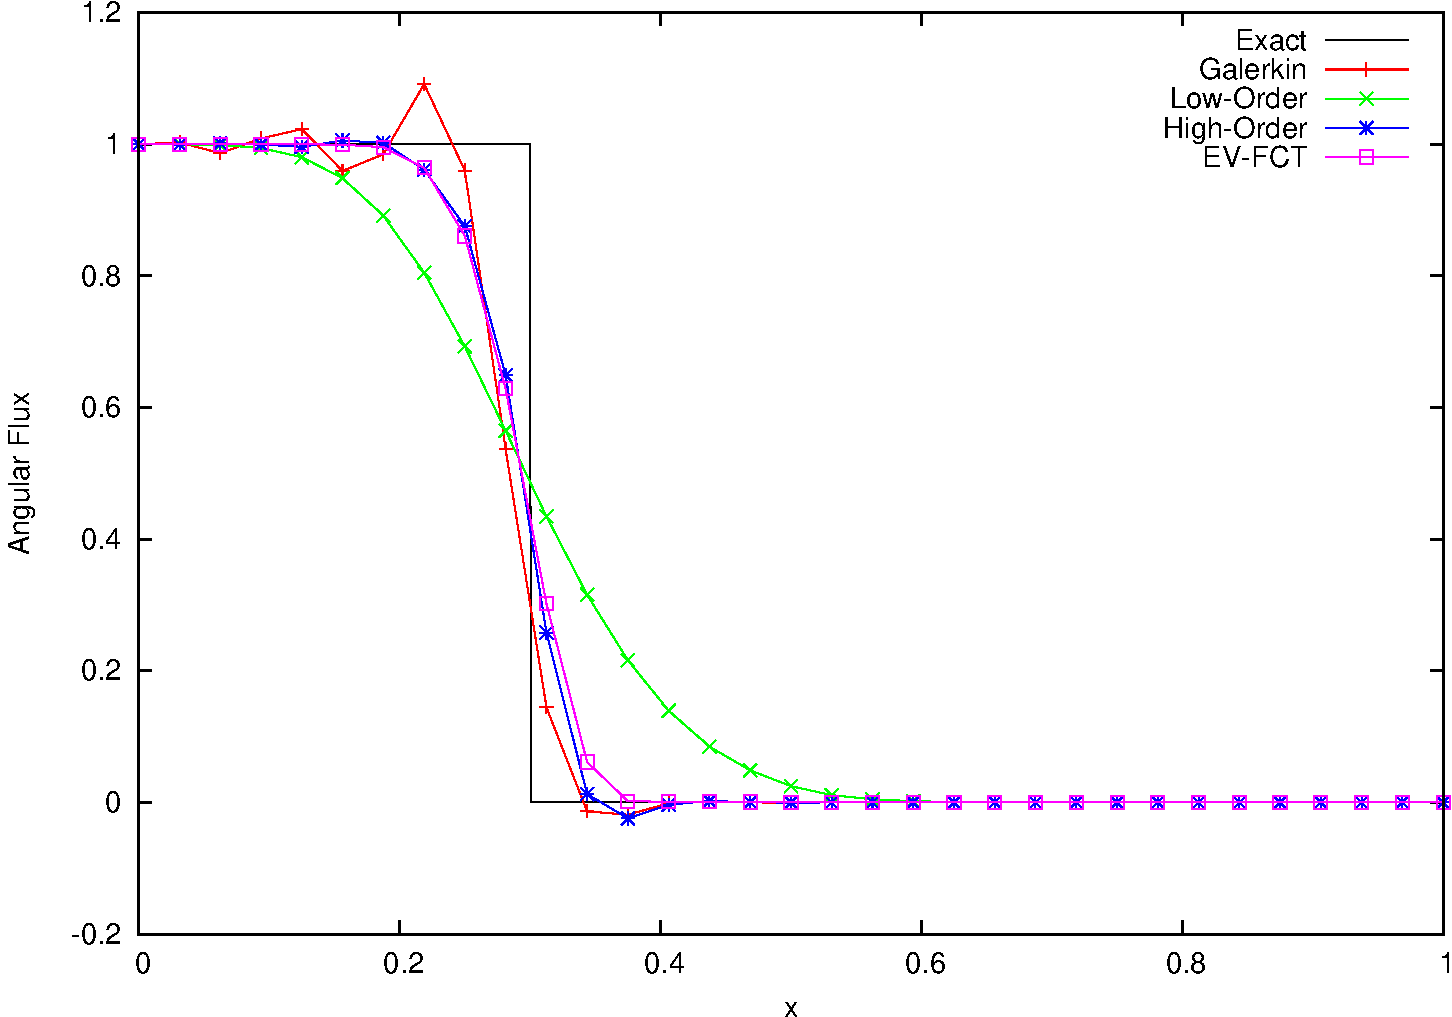
\includegraphics[width=\textwidth]{./figures/advection_FCT.pdf}

\end{frame}
%%%%%%%%%%%%%%%%%%%%%%%%%%%%%%%%%%%%%%%%%%%%%%%%%%%%%%%%%%%%%%%%%%%%%%%%%%%%%%%%%%%%%%%%%%%%%
\section{Results}
\begin{frame}
\frametitle{Results}
\framesubtitle{Source Problem Results}

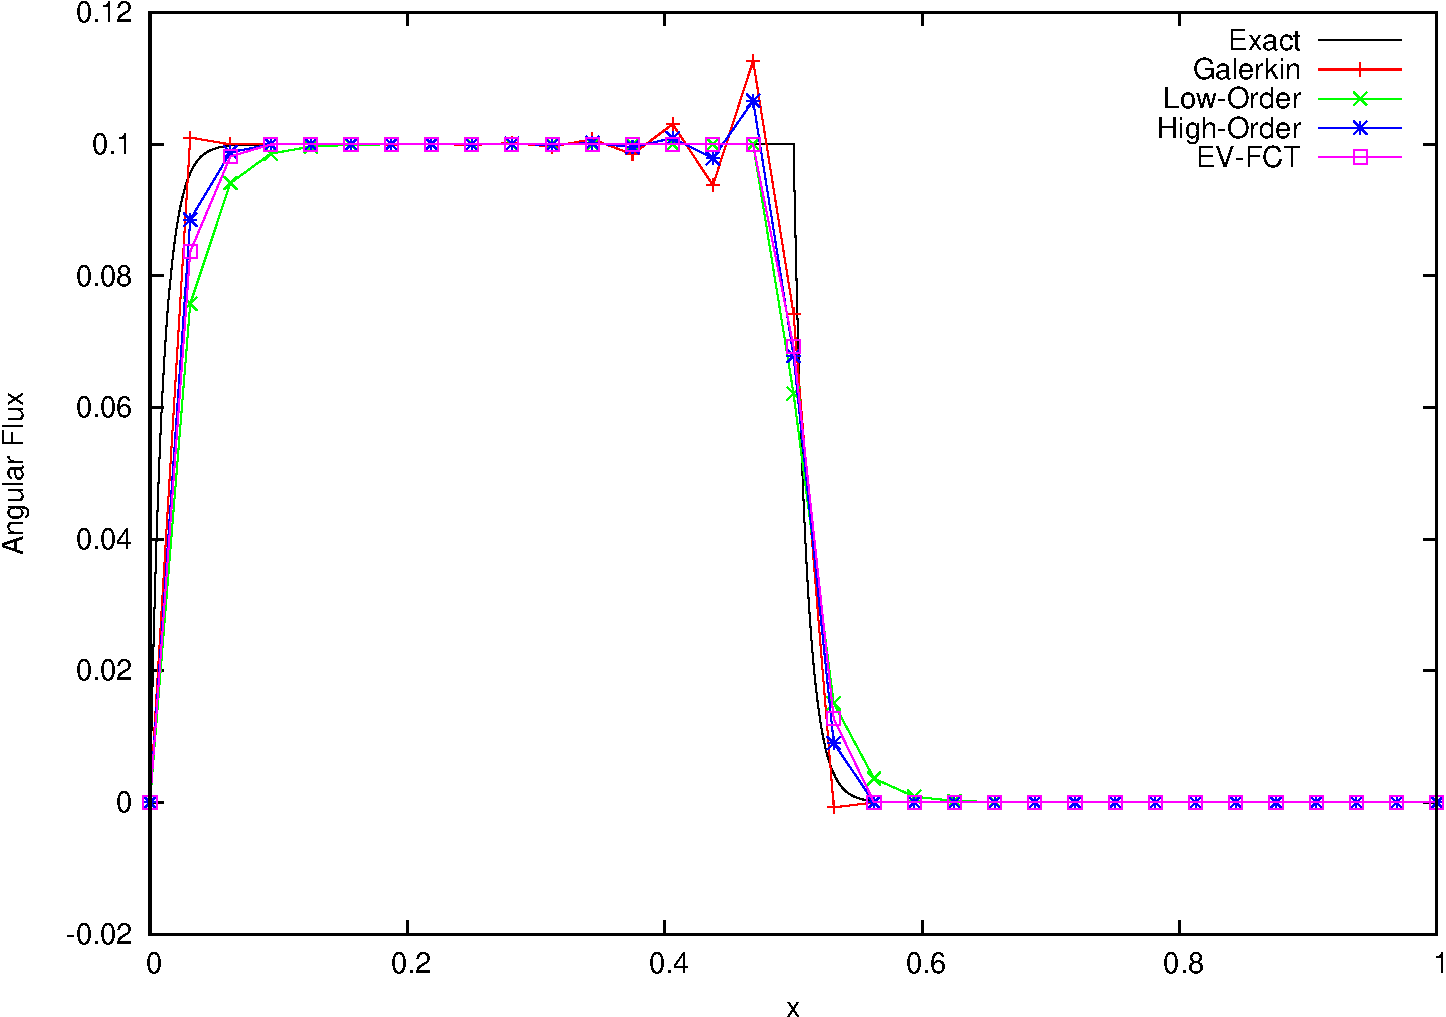
\includegraphics[width=\textwidth]{./figures/solutions_source_FE.pdf}

\end{frame}
%%%%%%%%%%%%%%%%%%%%%%%%%%%%%%%%%%%%%%%%%%%%%%%%%%%%%%%%%%%%%%%%%%%%%%%%%%%%%%%%%%%%%%%%%%%%%
\begin{frame}
\frametitle{Results}
\framesubtitle{Smooth Problem Convergence Results (Using FE)}

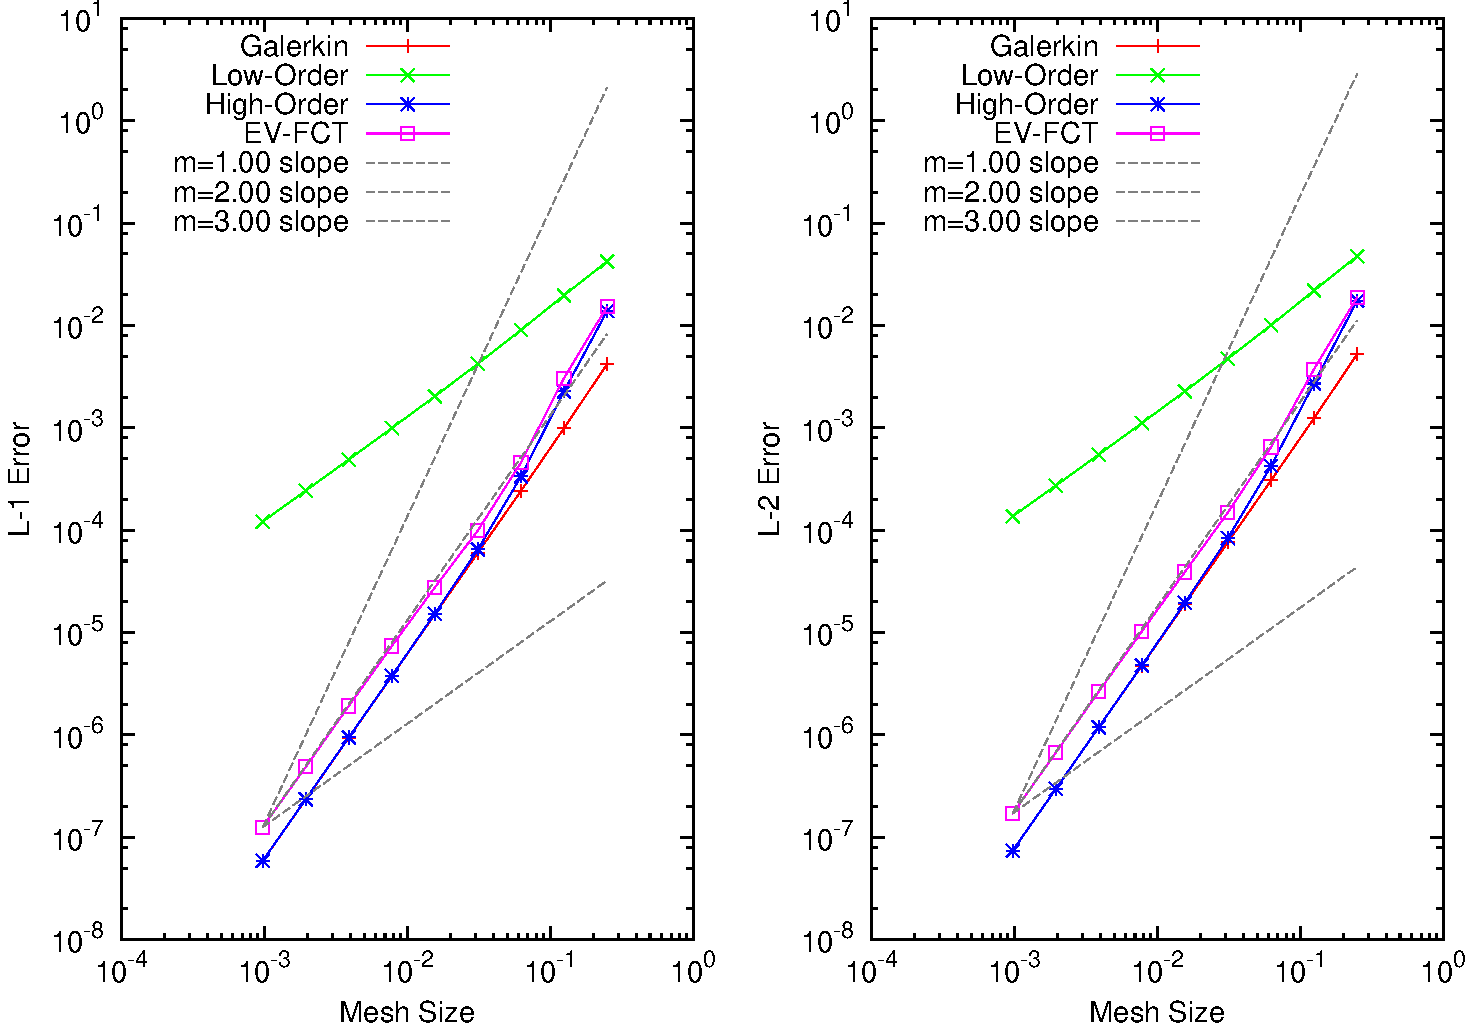
\includegraphics[width=\textwidth]{./figures/convergence_smooth_FE.pdf}

\end{frame}
%%%%%%%%%%%%%%%%%%%%%%%%%%%%%%%%%%%%%%%%%%%%%%%%%%%%%%%%%%%%%%%%%%%%%%%%%%%%%%%%%%%%%%%%%%%%%
\begin{frame}
\frametitle{Results}
\framesubtitle{Non-smooth Problem Convergence Results (Using SSPRK33)}

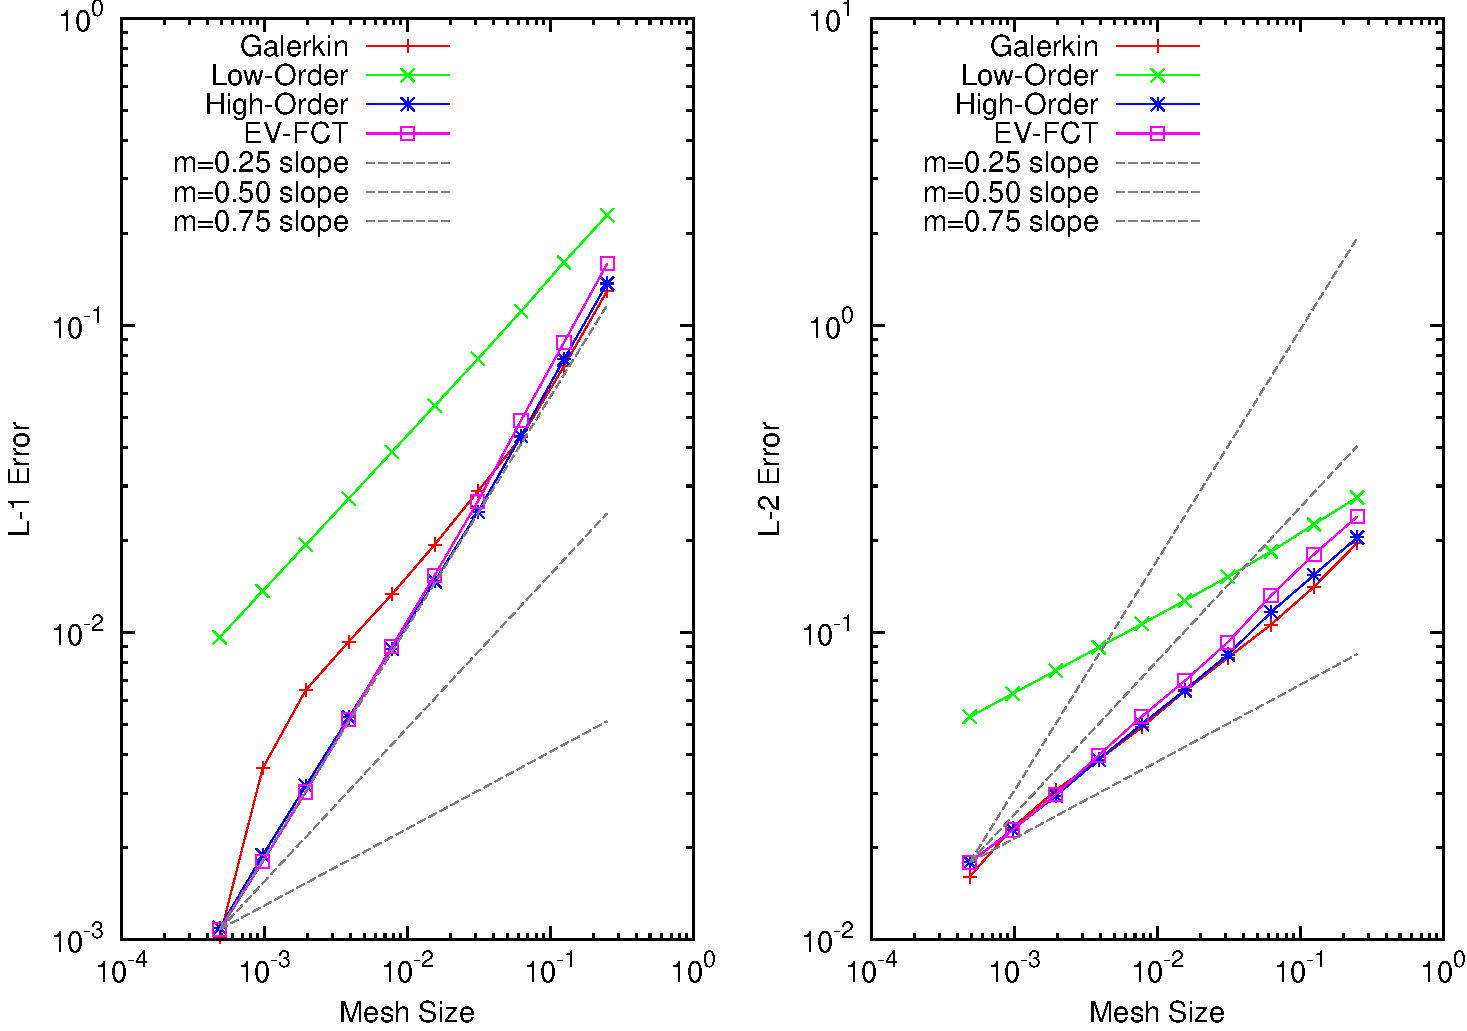
\includegraphics[width=\textwidth]{./figures/convergence_absorber_SSPRK33.pdf}

\end{frame}
%%%%%%%%%%%%%%%%%%%%%%%%%%%%%%%%%%%%%%%%%%%%%%%%%%%%%%%%%%%%%%%%%%%%%%%%%%%%%%%%%%%%%%%%%%%%%
\section{Conclusions}
\begin{frame}
\frametitle{Conclusions}

\begin{itemize}
   \item guaranteed non-negative, DMP-satisfying scheme
   \item monotonicity for problems tested, but not guaranteed
   \item theoretical convergence rates observed
   \item future work:
      \begin{itemize}
         \item implicit time discretizations
         \item steady-state
         \item more complicated physics
      \end{itemize}
\end{itemize}

\end{frame}
%%%%%%%%%%%%%%%%%%%%%%%%%%%%%%%%%%%%%%%%%%%%%%%%%%%%%%%%%%%%%%%%%%%%%%%%%%%%%%%%%%%%%%%%%%%%%
\begin{frame}
\frametitle{Acknowledgments}

\begin{itemize}
   \item Dr. Jean Ragusa, my advisor
   \item Dr. Jean-Luc Guermond, our collaborator and pioneer of the entropy-based artificial viscosity method
   \item Dr. Dmitri Kuzmin, an expert in FCT
\end{itemize}
\begin{itemize}
   \item This material is based upon work supported under an Integrated University Program Graduate Fellowship.
\end{itemize}

	\begin{center}
		
\includegraphics[width=0.4\textwidth]{./figures/NEUP_Final_Logo_Version-09.jpg}
	\end{center}
\end{frame}
%%%%%%%%%%%%%%%%%%%%%%%%%%%%%%%%%%%%%%%%%%%%%%%%%%%%%%%%%%%%%%%%%%%%%%%%%%%%%%%%%%%%%%%%%%%%%
\end{document}
